\documentclass[11pt,a4paper]{article}

\usepackage[utf8]{inputenc}
\usepackage[english]{babel}
\usepackage[T1]{fontenc}
\usepackage{lmodern}
\usepackage[hidelinks]{hyperref}
\usepackage{subcaption}
\usepackage{graphicx}

\usepackage{amsmath,amssymb,amsfonts}

\title{Vision and Image Processing\\Assignment 3}
\author{Malte Stær Nissen \\ \texttt{tgq958} \and Benjamin Braithwaite \\
\texttt{cpg608}}

\begin{document}
\maketitle

Image url: http://cdn.logicspot.com/wp-content/uploads/2011/11/Online-Competitor-Analysis.jpg
\url{http://www.korthalsaltes.com/photo/cubic_shapes/cubic_shape01.jpg}

Interpolation: http://www.mathworks.se/help/matlab/ref/interp1.html

\section{External force derivatives}
%
We compute the derivatives of the two expressions for computing the external force image $F$. This is related to the external energy term $E_\mathcal{E}$ by $E_\mathcal{E}(C) = \sum_{i=1}^n F(C(i))$.
\begin{itemize}
\item Local maxima of gradient magnitude:
\end{itemize}
%
\begin{align}
F &= - \frac12 \| g_\sigma \star \nabla I \|^2 \\
&= - \frac12 \| \nabla I_{\sigma} \|^2 \\
&= - \frac12 (\nabla I_{\sigma x}^2 + \nabla I_{\sigma y}^2)
\end{align}
%
We use the chain rule:
%
\begin{align}
F_x &= - (\nabla I_{\sigma x} \nabla I_{\sigma xx} + \nabla I_{\sigma y} \nabla I_{\sigma xy}) \\
F_y &= - (\nabla I_{\sigma x} \nabla I_{\sigma xy} + \nabla I_{\sigma y} \nabla I_{\sigma yy})
\end{align}
%
\begin{itemize}
\item Zero-crossings of Laplacian of Gaussian:
\end{itemize}
%
\begin{align}
F &= - \frac12 ( g_\sigma \star \Delta I)^2 \\
&= - \frac12 \Delta I_{\sigma}^2 \\
&= - \frac12 (\nabla I_{\sigma xx} + \nabla I_{\sigma yy})^2
\end{align}
%
We use the chain rule:
%
\begin{align}
F_x &= - (\nabla I_{\sigma xx} + \nabla I_{\sigma yy}) (\nabla I_{\sigma xxx} + \nabla I_{\sigma xyy}) \\
F_y &= - (\nabla I_{\sigma xx} + \nabla I_{\sigma yy}) (\nabla I_{\sigma xxy} + \nabla I_{\sigma yyy})
\end{align}
%

\section{Implementation description}
%
Our implementation is based on computing
%
\begin{align}
\mathbf{x}^{s+1} &= \mathbf{M}^{-1} (\mathbf{x} - \gamma F_x(\mathbf{x}^s, \mathbf{y}^s)), \\
\mathbf{y}^{s+1} &= \mathbf{M}^{-1} (\mathbf{y} - \gamma F_y(\mathbf{x}^s, \mathbf{y}^s))
\end{align}
%
for each iteration, as derived in the slides from gradient descent and the three energy terms. $\mathbf{M}$ is the system matrix and is constructed based on $\alpha$, $\beta$, and $\tau$. We halt the algorithm when the change in every point on the curve is less than some threshold $t$, or when a maximal number of iterations is reached. The parameters have the following function:
%
\begin{itemize}
\item $\alpha$: Weight of curve energy term, which minimizes the length of the curve.
\item $\beta$: Weight of bending energy term, which minimizes the bend between consecutive segments.
\item $\gamma$: Weight of the external energy term, which minimizes the external force of the image at the curve points.
\item $\tau$: Step size of one gradient descent iteration.
\end{itemize}
%
\section{Tests and examples}
%
We have chosen two images $\texttt{coins.png}$ and $\texttt{cubic.jpg}$, where the cubic image is slightly harder to segment than the coins image. For each image we have experimented with various parameters for both external energy terms, and found some that work the best. The results are shown in figures ...
%
\begin{figure}[H]
    \centering
    \begin{subfigure}[t]{0.48\textwidth}
        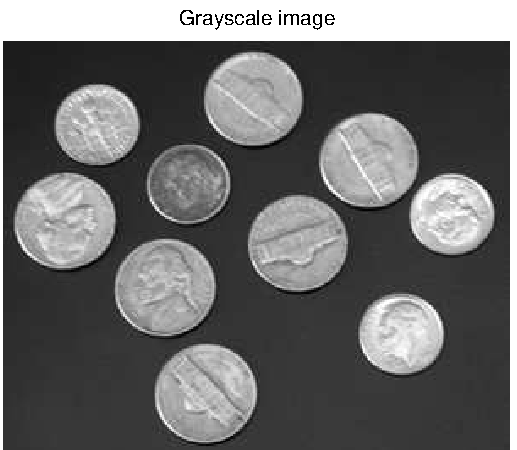
\includegraphics[width=\textwidth]{src/images/coins_gradient_gray.pdf}
        \caption{original image}
        \label{fig:coins_original}
    \end{subfigure}
    \begin{subfigure}[t]{0.48\textwidth}
        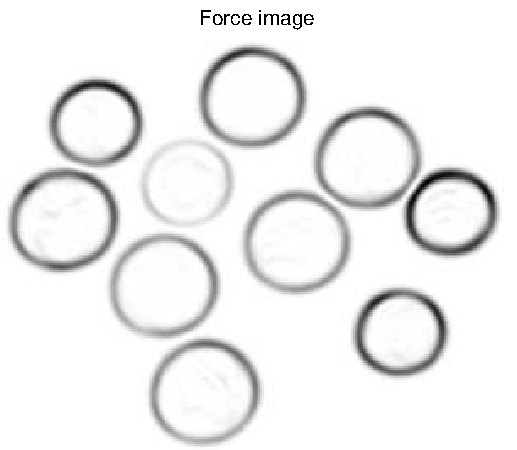
\includegraphics[width=\textwidth]{src/images/coins_gradient_forces.pdf}
        \caption{Force image}
        \label{fig:coins_forces}
    \end{subfigure}
    \begin{subfigure}[t]{0.48\textwidth}
        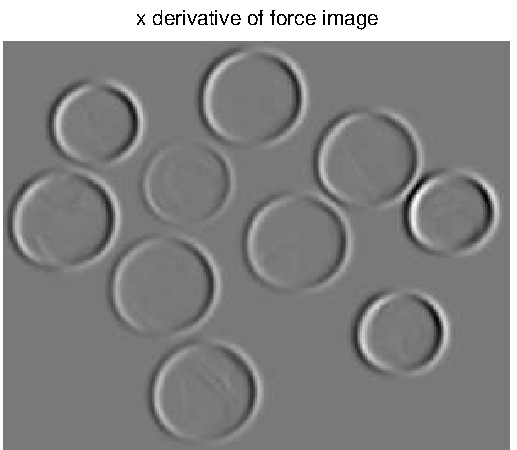
\includegraphics[width=\textwidth]{src/images/coins_gradient_xforces.pdf}
        \caption{x derivative of force image}
        \label{fig:coins_fx}
    \end{subfigure}
    \begin{subfigure}[t]{0.48\textwidth}
        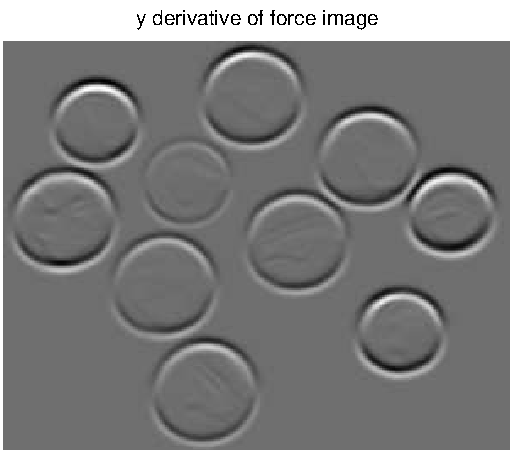
\includegraphics[width=\textwidth]{src/images/coins_gradient_yforces.pdf}
        \caption{y derivative of force image}
        \label{fig:coins_fy}
    \end{subfigure}
    \caption{\texttt{cubic.jpg} image and derivatives using $\sigma = 2$.}
    \label{fig:coins}
\end{figure}

\begin{figure}[H]
    \centering
    \caption{\texttt{cubic.jpg} image and derivatives using $\sigma = 2$.}
    \label{fig:cubic}
\end{figure}

\begin{figure}[H]
    \centering
    \begin{subfigure}[t]{0.48\textwidth}
        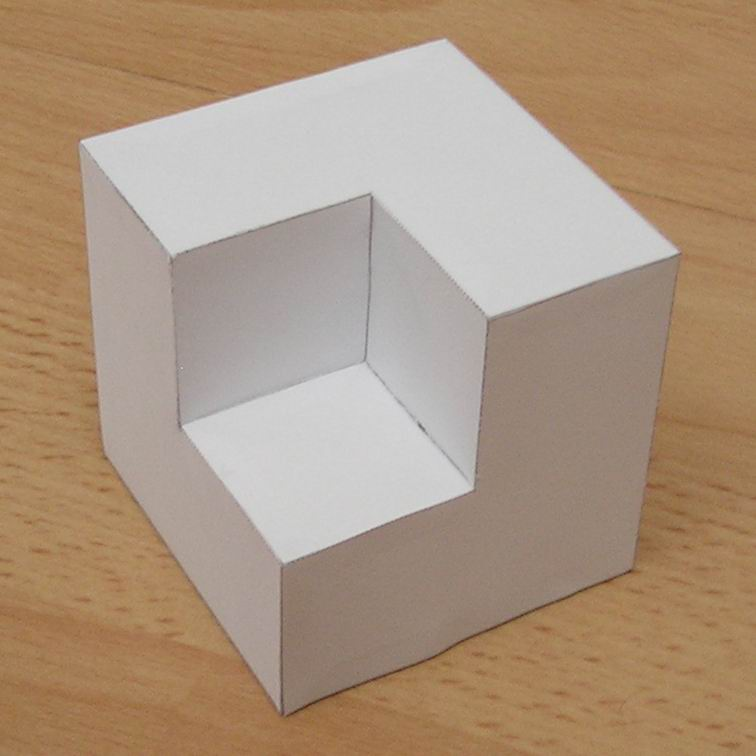
\includegraphics[width=\textwidth]{src/images/cubic_shape01.jpg}
        \caption{original image}
        \label{fig:cubic_original}
    \end{subfigure}
    \begin{subfigure}[t]{0.48\textwidth}
        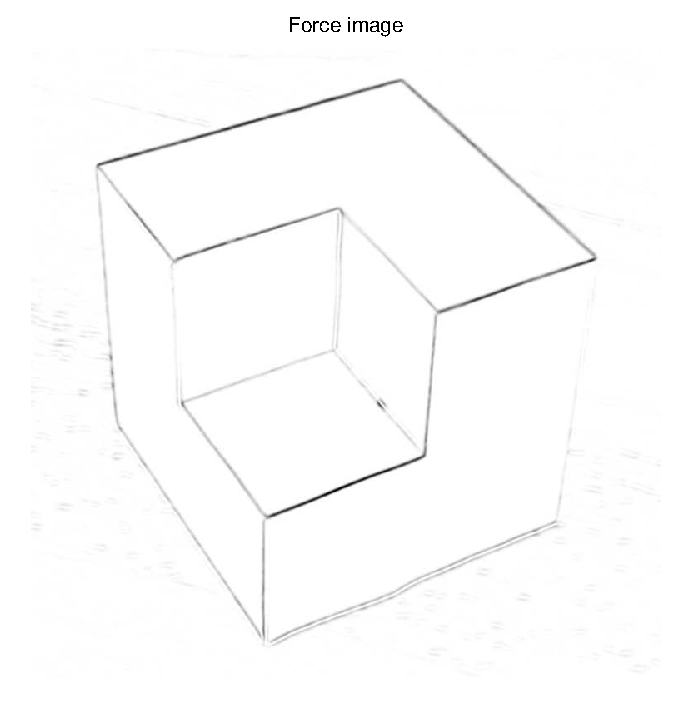
\includegraphics[width=\textwidth]{src/images/cubic_forces.pdf}
        \caption{Force image}
        \label{fig:cubic_forces}
    \end{subfigure}
    \begin{subfigure}[t]{0.48\textwidth}
        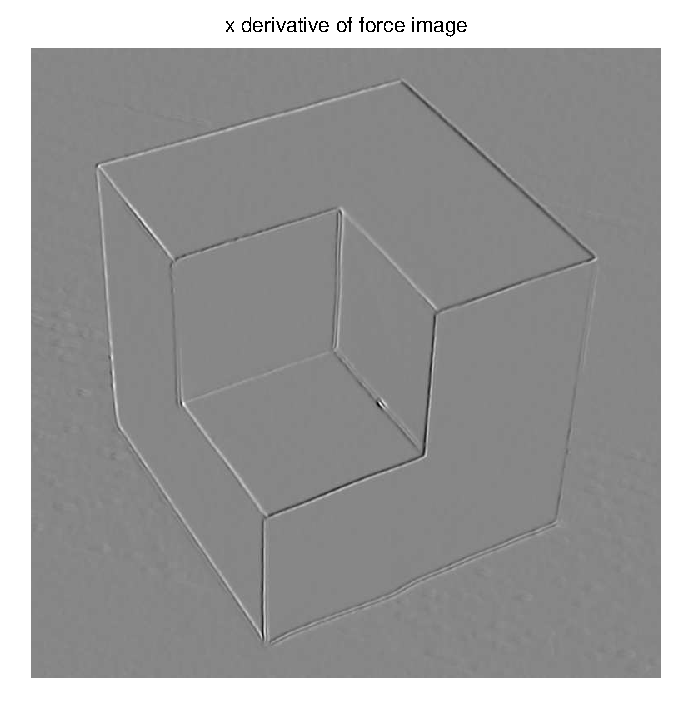
\includegraphics[width=\textwidth]{src/images/cubic_xforces.pdf}
        \caption{x derivative of force image}
        \label{fig:cubic_fx}
    \end{subfigure}
    \begin{subfigure}[t]{0.48\textwidth}
        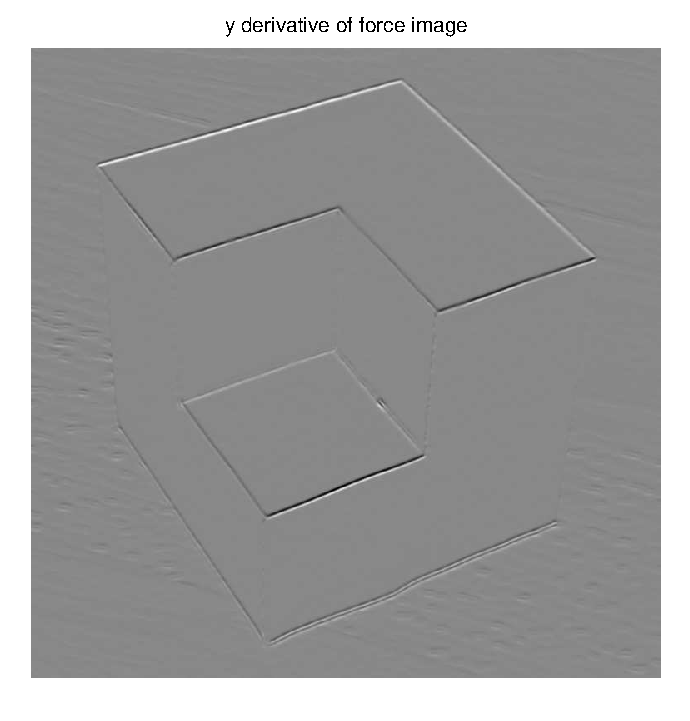
\includegraphics[width=\textwidth]{src/images/cubic_yforces.pdf}
        \caption{y derivative of force image}
        \label{fig:cubic_fy}
    \end{subfigure}
    \begin{subfigure}[t]{0.24\textwidth}
        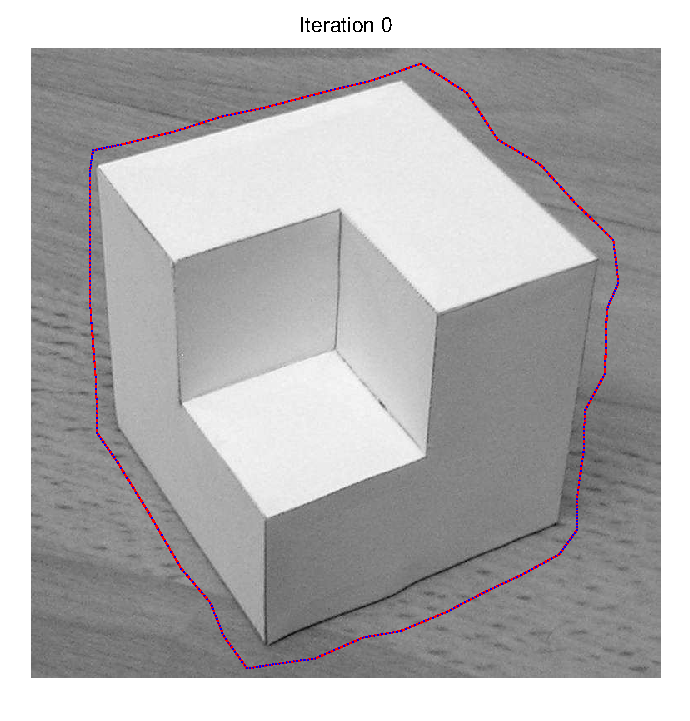
\includegraphics[width=\textwidth]{src/images/cubic_0.pdf}
        \caption{Snake start}
        \label{fig:cubic_grayscale}
    \end{subfigure}
    \begin{subfigure}[t]{0.24\textwidth}
        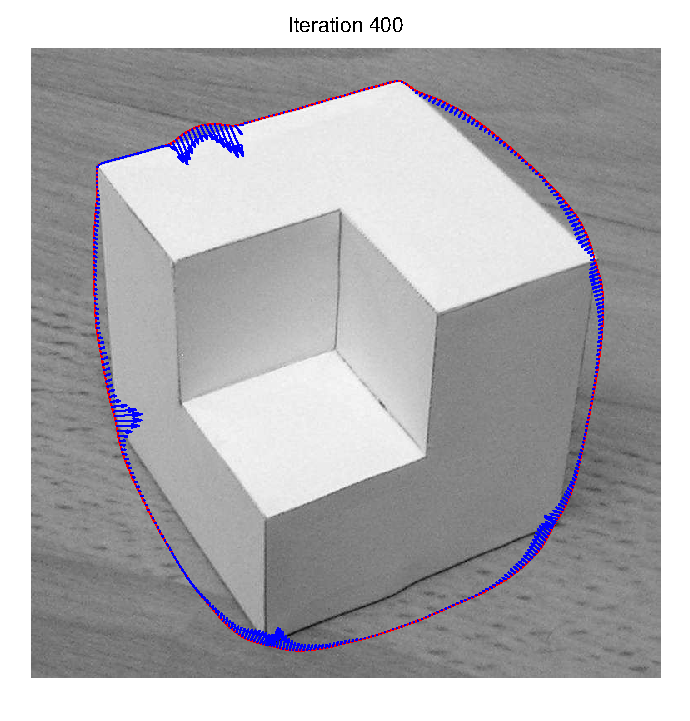
\includegraphics[width=\textwidth]{src/images/cubic_400.pdf}
        \caption{iteration 400}
        \label{fig:cubic_400}
    \end{subfigure}
    \begin{subfigure}[t]{0.24\textwidth}
        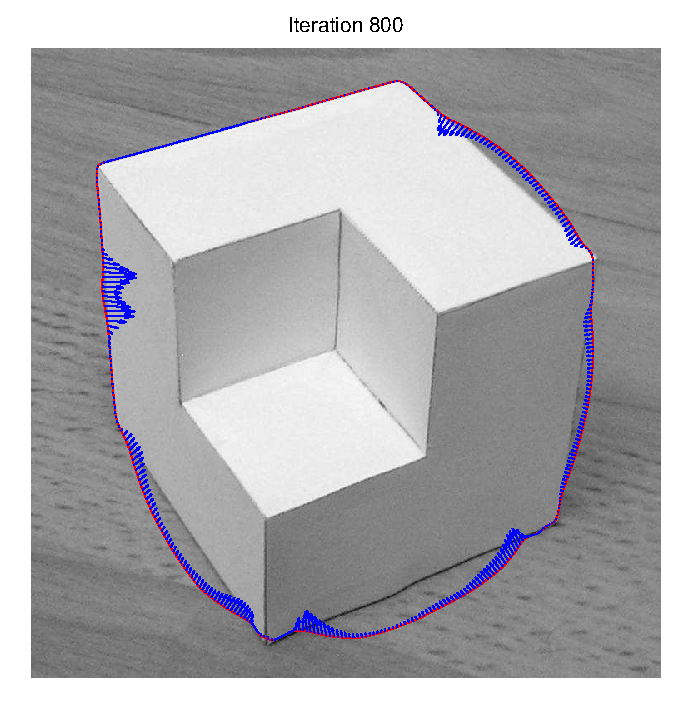
\includegraphics[width=\textwidth]{src/images/cubic_800.pdf}
        \caption{iteration 800}
        \label{fig:cubic_800}
    \end{subfigure}
    \begin{subfigure}[t]{0.24\textwidth}
        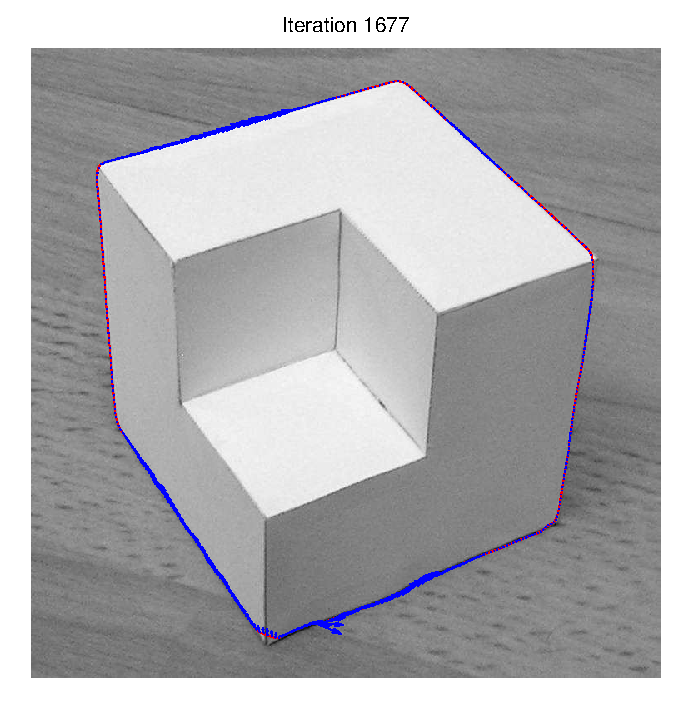
\includegraphics[width=\textwidth]{src/images/cubic_1677.pdf}
        \caption{snake stop (iteration 1677)}
        \label{fig:cubic_end}
    \end{subfigure}
    \caption{\texttt{cubic.jpg} snake intermediate results using setup: $\alpha
= 0.7$, $\beta = 0.5$, $\gamma = 1500$, $\tau = 0.4$, $\sigma = 2$.}
    \label{fig:cubic_intermediate}
\end{figure}

\end{document}

